%===============================================================================
% LaTeX sjabloon voor de bachelorproef toegepaste informatica aan HOGENT
% Meer info op https://github.com/HoGentTIN/latex-hogent-report
%===============================================================================

\documentclass[dutch,dit,thesis]{hogentreport}

% TODO:
% - If necessary, replace the option `dit`' with your own department!
%   Valid entries are dbo, dbt, dgz, dit, dlo, dog, dsa, soa
% - If you write your thesis in English (remark: only possible after getting
%   explicit approval!), remove the option "dutch," or replace with "english".

\usepackage{lipsum} % For blind text, can be removed after adding actual content

%% Pictures to include in the text can be put in the graphics/ folder
\graphicspath{{graphics/}}

%% For source code highlighting, requires pygments to be installed
%% Compile with the -shell-escape flag!
\usepackage[section]{minted}
%% If you compile with the make_thesis.{bat,sh} script, use the following
%% import instead:
%% \usepackage[section,outputdir=../output]{minted}
\usemintedstyle{solarized-light}
\definecolor{bg}{RGB}{253,246,227} %% Set the background color of the codeframe

%% Change this line to edit the line numbering style:
\renewcommand{\theFancyVerbLine}{\ttfamily\scriptsize\arabic{FancyVerbLine}}

%% Macro definition to load external java source files with \javacode{filename}:
\newmintedfile[javacode]{java}{
    bgcolor=bg,
    fontfamily=tt,
    linenos=true,
    numberblanklines=true,
    numbersep=5pt,
    gobble=0,
    framesep=2mm,
    funcnamehighlighting=true,
    tabsize=4,
    obeytabs=false,
    breaklines=true,
    mathescape=false
    samepage=false,
    showspaces=false,
    showtabs =false,
    texcl=false,
}

% Other packages not already included can be imported here

%%---------- Document metadata -------------------------------------------------
% TODO: Replace this with your own information
\author{Ernst Aarden}
\supervisor{Dhr. F. Van Houte}
\cosupervisor{Mevr. S. Beeckman}
\title[Optionele ondertitel]%
    {Titel van de bachelorproef}
\academicyear{\advance\year by -1 \the\year--\advance\year by 1 \the\year}
\examperiod{1}
\degreesought{\IfLanguageName{dutch}{Professionele bachelor in de toegepaste informatica}{Bachelor of applied computer science}}
\partialthesis{false} %% To display 'in partial fulfilment'
%\institution{Internshipcompany BVBA.}

%% Add global exceptions to the hyphenation here
\hyphenation{back-slash}

%% The bibliography (style and settings are  found in hogentthesis.cls)
\addbibresource{bachproef.bib}            %% Bibliography file
\addbibresource{../voorstel/voorstel.bib} %% Bibliography research proposal
\defbibheading{bibempty}{}

%% Prevent empty pages for right-handed chapter starts in twoside mode
\renewcommand{\cleardoublepage}{\clearpage}

\renewcommand{\arraystretch}{1.2}

%% Content starts here.
\begin{document}

%---------- Front matter -------------------------------------------------------

\frontmatter

\hypersetup{pageanchor=false} %% Disable page numbering references
%% Render a Dutch outer title page if the main language is English
\IfLanguageName{english}{%
    %% If necessary, information can be changed here
    \degreesought{Professionele Bachelor toegepaste informatica}%
    \begin{otherlanguage}{dutch}%
       \maketitle%
    \end{otherlanguage}%
}{}

%% Generates title page content
\maketitle
\hypersetup{pageanchor=true}

%%=============================================================================
%% Voorwoord
%%=============================================================================

\chapter*{\IfLanguageName{dutch}{Woord vooraf}{Preface}}%
\label{ch:voorwoord}

%% TODO:
%% Het voorwoord is het enige deel van de bachelorproef waar je vanuit je
%% eigen standpunt (``ik-vorm'') mag schrijven. Je kan hier bv. motiveren
%% waarom jij het onderwerp wil bespreken.
%% Vergeet ook niet te bedanken wie je geholpen/gesteund/... heeft

Met deze bachelorproef sluit ik een 3-jarig hoofdstuk af, het hoofdstuk 
toegepaste informatica die ik volgde aan de Hogeschool Gent. Deze opleiding 
heeft mij voorbereid voor een toekomst als systeembeheerder, en in samenwerking 
met 
%%=============================================================================
%% Samenvatting
%%=============================================================================

% TODO: De "abstract" of samenvatting is een kernachtige (~ 1 blz. voor een
% thesis) synthese van het document.
%
% Een goede abstract biedt een kernachtig antwoord op volgende vragen:
%
% 1. Waarover gaat de bachelorproef?
% 2. Waarom heb je er over geschreven?
% 3. Hoe heb je het onderzoek uitgevoerd?
% 4. Wat waren de resultaten? Wat blijkt uit je onderzoek?
% 5. Wat betekenen je resultaten? Wat is de relevantie voor het werkveld?
%
% Daarom bestaat een abstract uit volgende componenten:
%
% - inleiding + kaderen thema
% - probleemstelling
% - (centrale) onderzoeksvraag
% - onderzoeksdoelstelling
% - methodologie
% - resultaten (beperk tot de belangrijkste, relevant voor de onderzoeksvraag)
% - conclusies, aanbevelingen, beperkingen
%
% LET OP! Een samenvatting is GEEN voorwoord!

%%---------- Nederlandse samenvatting -----------------------------------------
%
% TODO: Als je je bachelorproef in het Engels schrijft, moet je eerst een
% Nederlandse samenvatting invoegen. Haal daarvoor onderstaande code uit
% commentaar.
% Wie zijn bachelorproef in het Nederlands schrijft, kan dit negeren, de inhoud
% wordt niet in het document ingevoegd.

\IfLanguageName{english}{%
\selectlanguage{dutch}
\chapter*{Samenvatting}
\lipsum[1-4]
\selectlanguage{english}
}{}

%%---------- Samenvatting -----------------------------------------------------
% De samenvatting in de hoofdtaal van het document

\chapter*{\IfLanguageName{dutch}{Samenvatting}{Abstract}}

\lipsum[1-4]


%---------- Inhoud, lijst figuren, ... -----------------------------------------

\tableofcontents

% In a list of figures, the complete caption will be included. To prevent this,
% ALWAYS add a short description in the caption!
%
%  \caption[short description]{elaborate description}
%
% If you do, only the short description will be used in the list of figures

\listoffigures

% If you included tables and/or source code listings, uncomment the appropriate
% lines.
%\listoftables
%\listoflistings

% Als je een lijst van afkortingen of termen wil toevoegen, dan hoort die
% hier thuis. Gebruik bijvoorbeeld de ``glossaries'' package.
% https://www.overleaf.com/learn/latex/Glossaries

%---------- Kern ---------------------------------------------------------------

\mainmatter{}

% De eerste hoofdstukken van een bachelorproef zijn meestal een inleiding op
% het onderwerp, literatuurstudie en verantwoording methodologie.
% Aarzel niet om een meer beschrijvende titel aan deze hoofdstukken te geven of
% om bijvoorbeeld de inleiding en/of stand van zaken over meerdere hoofdstukken
% te verspreiden!

%%=============================================================================
%% Inleiding
%%=============================================================================

\chapter{\IfLanguageName{dutch}{Inleiding}{Introduction}}%
\label{ch:inleiding}

De inleiding moet de lezer net genoeg informatie verschaffen om het onderwerp te begrijpen en in te zien waarom de onderzoeksvraag de moeite waard is om te onderzoeken. In de inleiding ga je literatuurverwijzingen beperken, zodat de tekst vlot leesbaar blijft. Je kan de inleiding verder onderverdelen in secties als dit de tekst verduidelijkt. Zaken die aan bod kunnen komen in de inleiding~\autocite{Pollefliet2011}:

\begin{itemize}
  \item context, achtergrond
  \item afbakenen van het onderwerp
  \item verantwoording van het onderwerp, methodologie
  \item probleemstelling
  \item onderzoeksdoelstelling
  \item onderzoeksvraag
  \item \ldots
\end{itemize}

\section{\IfLanguageName{dutch}{Probleemstelling}{Problem Statement}}%
\label{sec:probleemstelling}

Uit je probleemstelling moet duidelijk zijn dat je onderzoek een meerwaarde heeft voor een concrete doelgroep. De doelgroep moet goed gedefinieerd en afgelijnd zijn. Doelgroepen als ``bedrijven,'' ``KMO's'', systeembeheerders, enz.~zijn nog te vaag. Als je een lijstje kan maken van de personen/organisaties die een meerwaarde zullen vinden in deze bachelorproef (dit is eigenlijk je steekproefkader), dan is dat een indicatie dat de doelgroep goed gedefinieerd is. Dit kan een enkel bedrijf zijn of zelfs één persoon (je co-promotor/opdrachtgever).

\section{\IfLanguageName{dutch}{Onderzoeksvraag}{Research question}}%
\label{sec:onderzoeksvraag}

Wees zo concreet mogelijk bij het formuleren van je onderzoeksvraag. Een onderzoeksvraag is trouwens iets waar nog niemand op dit moment een antwoord heeft (voor zover je kan nagaan). Het opzoeken van bestaande informatie (bv. ``welke tools bestaan er voor deze toepassing?'') is dus geen onderzoeksvraag. Je kan de onderzoeksvraag verder specifiëren in deelvragen. Bv.~als je onderzoek gaat over performantiemetingen, dan 

\section{\IfLanguageName{dutch}{Onderzoeksdoelstelling}{Research objective}}%
\label{sec:onderzoeksdoelstelling}

Wat is het beoogde resultaat van je bachelorproef? Wat zijn de criteria voor succes? Beschrijf die zo concreet mogelijk. Gaat het bv.\ om een proof-of-concept, een prototype, een verslag met aanbevelingen, een vergelijkende studie, enz.

\section{\IfLanguageName{dutch}{Opzet van deze bachelorproef}{Structure of this bachelor thesis}}%
\label{sec:opzet-bachelorproef}

% Het is gebruikelijk aan het einde van de inleiding een overzicht te
% geven van de opbouw van de rest van de tekst. Deze sectie bevat al een aanzet
% die je kan aanvullen/aanpassen in functie van je eigen tekst.

De rest van deze bachelorproef is als volgt opgebouwd:

In Hoofdstuk~\ref{ch:stand-van-zaken} wordt een overzicht gegeven van de stand van zaken binnen het onderzoeksdomein, op basis van een literatuurstudie.

In Hoofdstuk~\ref{ch:methodologie} wordt de methodologie toegelicht en worden de gebruikte onderzoekstechnieken besproken om een antwoord te kunnen formuleren op de onderzoeksvragen.

% TODO: Vul hier aan voor je eigen hoofstukken, één of twee zinnen per hoofdstuk

In Hoofdstuk~\ref{ch:conclusie}, tenslotte, wordt de conclusie gegeven en een antwoord geformuleerd op de onderzoeksvragen. Daarbij wordt ook een aanzet gegeven voor toekomstig onderzoek binnen dit domein.
\chapter{\IfLanguageName{dutch}{Stand van zaken}{State of the art}}%
\label{ch:stand-van-zaken}

% Tip: Begin elk hoofdstuk met een paragraaf inleiding die beschrijft hoe
% dit hoofdstuk past binnen het geheel van de bachelorproef. Geef in het
% bijzonder aan wat de link is met het vorige en volgende hoofdstuk.

% Pas na deze inleidende paragraaf komt de eerste sectiehoofding.

%Dit hoofdstuk bevat je literatuurstudie. De inhoud gaat verder op de inleiding, maar zal het onderwerp van de bachelorproef *diepgaand* uitspitten. De bedoeling is dat de lezer na lezing van dit hoofdstuk helemaal op de hoogte is van de huidige stand van zaken (state-of-the-art) in het onderzoeksdomein. Iemand die niet vertrouwd is met het onderwerp, weet nu voldoende om de rest van het verhaal te kunnen volgen, zonder dat die er nog andere informatie moet over opzoeken \autocite{Pollefliet2011}.

%Je verwijst bij elke bewering die je doet, vakterm die je introduceert, enz.\ naar je bronnen. In \LaTeX{} kan dat met het commando \texttt{$\backslash${textcite\{\}}} of \texttt{$\backslash${autocite\{\}}}. Als argument van het commando geef je de ``sleutel'' van een ``record'' in een bibliografische databank in het Bib\LaTeX{}-formaat (een tekstbestand). Als je expliciet naar de auteur verwijst in de zin (narratieve referentie), gebruik je \texttt{$\backslash${}textcite\{\}}. Soms is de auteursnaam niet expliciet een onderdeel van de zin, dan gebruik je \texttt{$\backslash${}autocite\{\}} (referentie tussen haakjes). Dit gebruik je bv.~bij een citaat, of om in het bijschrift van een overgenomen afbeelding, broncode, tabel, enz. te verwijzen naar de bron. In de volgende paragraaf een voorbeeld van elk.

%\textcite{Knuth1998} schreef een van de standaardwerken over sorteer- en zoekalgoritmen. Experten zijn het erover eens dat cloud computing een interessante opportuniteit vormen, zowel voor gebruikers als voor dienstverleners op vlak van informatietechnologie~\autocite{Creeger2009}.

%Let er ook op: het \texttt{cite}-commando voor de punt, dus binnen de zin. Je verwijst meteen naar een bron in de eerste zin die erop gebaseerd is, dus niet pas op het einde van een paragraaf.
\section{Ansible}
\subsection{Definitie}
\label{Definitie}
Ansible is een open-source automatiseringsplatform dat kan worden gebruikt om grote groepen computersystemen te beheren. 
Het helpt je bij het automatiseren van de implementatie van applicaties, configuratiebeheer, cloud provisioning, 
het updaten van werkstations en servers en vele andere taken. 
\par 
Ansible werkt op Windows en Unix systemen en is opgenomen 
als onderdeel van de Fedora distributie. Maar machines die gebruikt worden om de automatisering uit te voeren - 
controleknooppunten genoemd - moeten Unix/Linux systemen zijn. Je kunt Windows machines gebruiken, 
maar met een Windows Subsystem for Linux distributie. 
\par
Een van de meest opwindende aspecten van Ansible is dat het zonder 
agents werkt, in tegenstelling tot de meeste andere oplossingen voor configuratiebeheer. 
Het vereist geen systemen op afstand met een specifieke agent of software om wijzigingen 
aan te brengen of opdrachten uit te voeren
\autocite{Manjaly2022}.

\subsection{Voordelen van Ansible}
\label{Voordelen van Ansible}

\begin{enumerate}
  \item Het vermindert de middelen die nodig zijn voor IT-beheer - Sysadmins kunnen honderden of zelfs duizenden machines 
  vanaf één punt en in één keer beheren.

  \item Het maakt automatisering toegankelijk - Een van de ontwerpdoelen van Ansible was dat er minimale kennis nodig zou zijn 
  om het te gebruiken. Het platform gebruikt YAML (Yet Another Markup Language), een voor mensen leesbare taal met elementen 
  uit andere gangbare programmeertalen.

  \item Het Ansible platform heeft geen invloed op de prestaties - Ansible vereist geen agents of software die op beheerde 
  systemen draait of geïnstalleerd is. Daarom hoeven beheerde systemen geen rekenkracht aan Ansible te besteden.

  \item Het zorgt voor consistentie - Het platform is ontworpen om minimaal te zijn en gebruikers in staat te stellen consistente 
  omgevingen te creëren. En de hele operatie verloopt via een SSH-verbinding, wat betekent dat het forum niet nog meer 
  complexiteit toevoegt aan de systemen
  \autocite{Manjaly2022}.
\end{enumerate}

\subsection{Ansible voor cloud automation}
\label{Ansible voor cloud automation}
Cloud provisioning is een cruciaal onderdeel van het moderne cloud computing-model. 
We leven in het tijdperk van microservices, waar automatisering geen nice-to-have meer is. 
Het is een integraal onderdeel geworden van de dagelijkse activiteiten.
\par
Gelukkig is er een grote verscheidenheid aan automatiserings- en orkestratietools. 
Deze tools kunnen ons tijd besparen en tegelijkertijd de prestaties en nauwkeurigheid van provisionerings- en 
configuratiebeheerprocessen verbeteren.
\par
Ansible is in de eerste plaats een automatiseringstool. Met de juiste inhoud (rollen, modules en andere plugins) kan Ansible bijna 
alles automatiseren. En cloudbeheer is geen uitzondering, wat betekent dat we onze provisioneringsprocessen met relatief gemak 
kunnen automatiseren.
\par
Met een beetje hulp van producten voor continue integratie en continue implementatie (CI/CD) kan Ansible veranderen in een 
machtige orkestratietool. We kunnen beginnen met het combineren van op zichzelf staande taken tot complexe workflows die 
complexe IT-processen automatiseren.
\par
En als we workflowuitvoeringen koppelen aan gebeurtenissen uit onze monitoringsystemen, 
hebben we een aantal serieuze stappen gezet in de richting van een zelfherstellende infrastructuur
\autocite{Borovšak2021}.

\section{AWS}
  \subsection{Definitie}
\label{Definitie}
Amazon Lightsail is een AWS dienst die virtual private server (VPS) instances, containers, opslag en beheerde databases biedt 
tegen een kosteneffectieve en voorspelbare maandelijkse prijs. Het is bedoeld als de eenvoudigste manier om aan de slag te 
gaan met AWS voor kleine bedrijven, studenten, ontwikkelaars en anderen die hun website of applicaties voor algemene doeleinden 
in de cloud willen hosten.
\par
Lightsail is ontworpen met eenvoud in het achterhoofd, waardoor het gemakkelijk is voor gebruikers om websites en 
applicaties te implementeren die misschien niet veel cloudervaring hebben. De eenvoudige interface biedt gebruikers een 
minimaal aantal opties om te configureren, zodat ze hun bronnen snel en betrouwbaar kunnen inzetten zonder extra kennis of 
AWS-ervaring
\autocite{Graf2022}.

\subsection{Waarom kiezen voor AWS?}
\label{Waarom kiezen voor AWS?}
Je betaalt geen extra kosten voor de manier waarop de infrastructuur is aangeschaft en gelicentieerd, 
en zodra je deze diensten niet meer gebruikt, schakel je het uit en betaal je er niet meer voor.
Hoewel er een aantal grote spelers op de markt zijn, waaronder Azure (Microsoft), Google Cloud, IBM Cloud en Oracle, 
was AWS op het moment van schrijven nog steeds de belangrijkste speler in de ruimte
\autocite{Sesto2022}.

\section{Infrastructure as Code (IaC)}
\subsection{Definitie}
\label{Definitie}
Het beheer van de infrastructuurvoorziening van SaaS-applicaties van bedrijven wordt geconfronteerd met verschillende uitdagingen, zoals configuratiedrift en de heterogeniteit van cloudproviders. Daarom worden Infrastructure-as-Code (IaC) technologieën gebruikt om de uitrol van SaaS-applicaties te automatiseren. IaC vergemakkelijkt de snelle uitrol van nieuwe versies van applicatie-infrastructuren zonder dat dit ten koste gaat van de kwaliteit of stabiliteit \autocite{Achar2021}.
\par
Het bouwen van infrastructuur is een evoluerend proces dat vaak herhaalde aanpassingen en verbeteringen vereist met betrekking tot aspecten als schaalbaarheid, prestaties, fouttolerantie en onderhoudbaarheid. In traditionele omgevingen was het bouwen en implementeren van infrastructuurcomponenten een handmatige en vervelende taak, wat leidde tot vertragingen en verminderde wendbaarheid van de organisatie. Met de opkomst van IaC worden infrastructuurcomponenten nu behandeld als louter softwareconstructies,  een code die door verschillende teams gedeeld kan worden. Volgens Sandobalin et al. wordt Infrastructure as Code (IaC) gedefinieerd als een benadering van infrastructuurautomatisering gebaseerd op ontwikkelings- en operationele (DevOps) praktijken die continue samenwerking tussen ontwikkelaars en operationele medewerkers bevorderen door middel van een reeks principes, technieken en tools om de levertijd van software te optimaliseren. Om deze definitie samen te vatten, voldoet een IaC-oplossing aan de volgende principes:
\begin{enumerate}
  \item Versiecontrole is een populair concept waarin elke release overeenkomt met een build van broncode die wordt onderhouden als een artefact met versiebeheer in de omgeving. In IaC wordt een soortgelijk principe toegepast om de infrastructuur en wijzigingen te beheren met behulp van versiebeheer-commits in de broncode-repository. Dit zorgt voor traceerbaarheid van veranderingen die zijn aangebracht in de infrastructuurdefinitie, met vermelding van wie veranderingen heeft aangebracht, wat er is veranderd, enzovoort. Dit is cruciaal bij het terugdraaien naar een vorige codeversie tijdens het oplossen van een probleem.

  \item Voorspelbaarheid verwijst naar de IaC-mogelijkheid als een oplossing om altijd dezelfde omgeving en bijbehorende attributen (zoals gedefinieerd in het versiebeheersysteem) te bieden elke keer dat deze wordt aangeroepen.

  \item Consistentie zorgt ervoor dat meerdere instanties van dezelfde basislijncode een vergelijkbare omgeving bieden.  Dit voorkomt inconsistenties en configuratiedrift bij het handmatig bouwen van complexe infrastructuureenheden.

  \item Repeatability is een oplossing die altijd dezelfde resultaten levert op basis van de input.

  \item Composability verwijst naar een service die wordt beheerd in een modulair en abstract formaat, dat kan worden gebruikt om complexe applicatiesystemen te bouwen. Deze eigenschap stelt gebruikers in staat om zich te concentreren op het bouwen van de doelapplicatie in plaats van zich zorgen te maken over de details onder de motorkap en de complexe logica die wordt gebruikt voor provisioning.
  \autocite{Achar2021}.
\end{enumerate}

\subsection{IaC Concepten}
\label{IaC Concepten}
\begin{enumerate}
    \item Elke infrastructuurbron/component wordt gedeclareerd als code, inclusief pakketten, mappen, gebruikersaccounts, hulpprogramma's en configuraties. 
    \item De broncode voor elke IaC tool wordt aangeduid met een specifieke term, bijv. packages, directories, user accounts, utilities, en configurations.
    \item IaC introduceert aspecten van herhaalbaarheid, aanzienlijke snelheidsverbeteringen en verhoogde betrouwbaarheid.
    \item -	IaC biedt consistentie in de build. Als je bijvoorbeeld verschillende omgevingen moet beheren (bijv. ontwikkeling, QA, staging en productie), zorgt het opstarten van die omgevingen vanuit dezelfde codebase ervoor dat de configuratiedrift tussen de omgevingen te verwaarlozen is, waardoor het domein gezond blijft.
    \autocite{Achar2021}.
\end{enumerate}

\subesection{Soorten IaC}
\label{Soorten IaC}
Een infrastructuurcodebase bevat veel aspecten, van het specificeren van infrastructuurbronnen tot het instellen van afzonderlijke instanties van andere gerelateerde bronnen tot het beheren van de levering van talloze onderling afhankelijke frameworkstukken.  Als gevolg hiervan zijn er verschillende technieken voor het beoordelen van verschillende soorten IaC.
\par
De meeste IaC tools ondersteunen twee primaire taalconstructies: imperatieve en declaratieve taal. Imperatieve code verwijst naar een procedurele reeks instructies die specificeren hoe een taak moet worden uitgevoerd. Ansible en Chef werken in een procedurele stijl, wat betekent dat ze stap-voor-stap codes identificeren en hoe de gewenste eindtoestand te bereiken. Aan de andere kant specificeert declaratieve code de gewenste eindtoestand, maar niet de methode om deze te voltooien. Bijvoorbeeld AWS CloudFormation, Google Deployment Manager, Terraform, SaltStack, Pulumi en Heat werken allemaal in een declaratieve codestijl. IaC moedigt een declaratieve codestijl aan waarin de gewenste eindtoestand en de configuratie aanwezig zijn voordat de uiteindelijke vorm wordt geleverd.  Declaratieve code is echter vaak beter herbruikbaar in de omgeving, omdat er rekening wordt gehouden met wijzigingen in de huidige configuratie en tegelijkertijd wordt voldaan aan elk nieuw verzoek voor nieuwe infrastructuur \autocite{Achar2021}.

\begin{figure}[!htb]
  \centering
  \includegraphics[width=\textwidth]{graphics/Declaratieve_code.png}
  \caption{Een bovenaanzicht van hoe declaratieve code werkt}
  \label{fig:gantt}
\end{figure}

\section{Production Information Managements System (PIMS)}
\subsection{Definitie}
\label{Definitie}

Product information management systems (PIMSs) zijn IT-systemen die worden gebruikt om klantgerichte productinformatie centraal te beheren en te synchroniseren. Ze richten zich op het verenigen en distribueren van productinformatie zonder de noodzaak van handmatige invoer in verschillende systemen. PIMS ondersteunen bedrijfsprocessen waarbij klantgerichte productinformatie betrokken is, zoals marketing. Ze bieden voordelen zoals een kortere time-to-market, een uitgebreider productassortiment, een uniforme klantervaring, beter complexiteitsbeheer, gecontroleerde distributie van content en naleving van wettelijke voorschriften. PIMS helpen ook bij het verlagen van de kosten, het verbeteren van de snelheid waarmee informatie wordt opgehaald, het minimaliseren van gegevensopschoning en logistieke fouten, en het verminderen van retourzendingen en informatieverzoeken.
\autocite{Battistello2021}
\par
Product Information Management (PIM) is een relatief nieuw begrip. Het concept begon rond 2003 aan kracht te winnen. Het wordt steeds populairder door de snelle groei van e-commerce en de populariteit van online winkels. In de eerste plaats vereist online verkoop dat bedrijven duidelijke basisproductinformatie verzamelen die consumenten ook echt kunnen begrijpen. Zonder productinformatie, zoals de naam van het product, de prijs en de productcategorie, kon het product helemaal niet online gevonden en verkocht worden. Ten tweede stelt het internet detail- en groothandelbedrijven in staat om veel meer producten online aan te bieden aan hun klanten, vaak omschreven als "long tail", dan in fysieke winkels.1 Terwijl het mogelijk was om productinformatie voor maximaal duizend of meer producten in een spreadsheet te beheren, bieden de meeste online winkels nu tienduizenden, zo niet honderdduizenden producten aan. In dit geval werken spreadsheets gewoon niet meer. Bovendien wordt productinformatie niet langer aangeboden via het web, maar via een grote verzameling kanalen zoals mobiele telefoons, tablets, winkels, verkooppunten, gedrukte catalogi, flyers, enz. Deze groei vraagt om een gespecialiseerd systeem om zoveel informatie te beheren die zo wijd verspreid is. Tegelijkertijd eisen consumenten meer, betere en consistente productinformatie. Over het algemeen geldt: hoe meer informatie, hoe meer je verkoopt. Een gedetailleerde productbeschrijving wordt gezien als een van de belangrijkste kenmerken van een webwinkel. Om een product online te verkopen willen klanten talloze details opzoeken en vergelijken en willen ze alle specificaties weten voordat ze kopen \autocite{Abraham2014}.
\par
Het belang van het PIM-systeem is toegenomen door de technische geavanceerdheid van producten, hun behoefte aan intern beheer of externe publicatie. ERP- en CCMS-systemen moeten worden geïntegreerd met een PIM-systeem dat fungeert als de "ruggengraat" van productinformatie \autocite{Matos2022}.

\begin{figure}[!htb]
  \centering
  \includegraphics[width=\textwidth]{bachproef/graphics/PIM_Definitie.jpg}
  \caption{PIM proces}
  \label{fig:PIM proces}
  \autocite{Derpunkt2021}
\end{figure}

\subsection{Voordelen van PIMS voor belanghebbenden}
\label{Voordelen van PIMS voor belanghebbenden}

De aspecten van het PIMS die relevant waren voor de belanghebbenden waren onder andere toegang hebben tot bijgewerkte productinformatie, het hebben van een gedeelde productinformatie HUB, het delen van informatie binnen het bedrijf en het definiëren van eigenaarschap en governance van productinformatie. De vereisten van de belanghebbenden werden geïdentificeerd met behulp van de MoSCoW-prioriteringstechniek. De startbijeenkomst hielp bij het vaststellen van een gemeenschappelijk begrip van de voordelen en beperkingen van PIMS en bij het verzamelen van de algemene problemen waarmee het bedrijf te maken had bij het beheren van productinformatie.
\autocite{Battistello2021}

\subsection{Voordelen van het stockeren van product information in PIMS}
\label{Voordelen van het stockeren van product information in PIMS}

Het opslaan van productinformatie in een PIMS biedt verschillende voordelen. Ten eerste helpt het om problemen met het beheer van productinformatie op te lossen en negatieve gevolgen voor het bedrijf te voorkomen. Ten tweede biedt het een gecentraliseerd en generiek model voor productinformatie, dat meestal niet direct beschikbaar is in bedrijven. Ten derde maakt het een gedeelde manier van het beheren van productinformatie mogelijk, wat vooral gunstig is voor organisaties met complexe structuren en meerdere belanghebbenden. Tot slot helpt het bij het definiëren en documenteren van de informatie die nodig is voor het project, waardoor het eenvoudiger wordt om belanghebbenden te betrekken en te zorgen voor duidelijkheid in het informatiebeheerproces.
\autocite{Battistello2021}

\subsection{Welke bedrijven komen in aanmerking?}
\label{Welke bedrijven komen in aanmerking?}
Een PIM-systeem is niet voor elk bedrijf een "must have". Verschillende factoren bepalen of er behoefte is aan een PIM-systeem:
\begin{enumerate}
    \item Veel producten en productwijzigingen: vooral modewinkels wijzigen hun hele assortiment twee keer of zelfs meer per jaar.
    \item Veel gebruikers: Excel is een geweldig hulpmiddel, maar met een paar duizend producten wordt het minder geweldig, vooral als meerdere mensen tegelijkertijd aan productinformatie moeten werken.
    \item Complexiteit van producten: wanneer producten veel kenmerken hebben en het soort producten dat wordt aangeboden sterk verschilt, nemen de kosten van het werken met Excel of standaard databasesystemen sterk toe. Met PIM-systemen kunnen producten veel eenvoudiger worden geclassificeerd.
    \item Gegevenskwaliteit/compliance: PIM heeft verschillende hulpmiddelen om de kwaliteit van productinformatie te verbeteren en te handhaven. Meestal wordt ook bijgehouden wie welke productinhoud bewerkt en/of goedkeurt en wanneer.
    \item Veel bronnen/synchronisaties: het handmatig importeren van gegevens is te doen als het gaat om het eens per week uploaden van een CSV-bestand. De dagelijkse synchronisatie van gegevens met 15 verschillende leveranciers kan echter het beste worden geautomatiseerd.
    \item Veel klantsegmenten: hoe meer klantsegmenten, hoe meer verschillende visies op het complete assortiment moeten worden onderhouden.
    \item Veel kanalen: hoe meer (verschillende) kanalen (print, web, mobiel, etc.) hoe waarschijnlijker het is dat verschillende outputformaten en interfaces ondersteund moeten worden.
    \item Landen/talen: als je productinformatie aanbiedt in 32 landen met lokale aanpassing van de inhoud, is een PIM niet langer een optie maar een must have. Zelfs bedrijven met een beperkt aantal producten kunnen besluiten om te investeren in een PIM-systeem. Een producent van premium kinderwagens heeft bijvoorbeeld maar drie verschillende soorten kinderwagens. De kinderwagens worden echter verkocht in meer dan 80 landen in 13 verschillende talen, de producten hebben meer dan 1000 varianten omdat onderdelen van kleur kunnen verschillen, productonderdelen na verloop van tijd veranderen en per land kunnen verschillen vanwege wettelijke eisen, enz. Als gevolg hiervan zijn meer dan 30 centrale marketingmedewerkers en lokale verkoopmedewerkers continu bezig met productinformatie en bleek een PIM-systeem noodzakelijk om de complexiteit te beheren \autocite{Abraham2014}.
\end{enumerate}


%%=============================================================================
%% Methodologie
%%=============================================================================

\chapter{\IfLanguageName{dutch}{Methodologie}{Methodology}}%
\label{ch:methodologie}

%% TODO: In dit hoofstuk geef je een korte toelichting over hoe je te werk bent
%% gegaan. Verdeel je onderzoek in grote fasen, en licht in elke fase toe wat
%% de doelstelling was, welke deliverables daar uit gekomen zijn, en welke
%% onderzoeksmethoden je daarbij toegepast hebt. Verantwoord waarom je
%% op deze manier te werk gegaan bent.
%% 
%% Voorbeelden van zulke fasen zijn: literatuurstudie, opstellen van een
%% requirements-analyse, opstellen long-list (bij vergelijkende studie),
%% selectie van geschikte tools (bij vergelijkende studie, "short-list"),
%% opzetten testopstelling/PoC, uitvoeren testen en verzamelen
%% van resultaten, analyse van resultaten, ...
%%
%% !!!!! LET OP !!!!!
%%
%% Het is uitdrukkelijk NIET de bedoeling dat je het grootste deel van de corpus
%% van je bachelorproef in dit hoofstuk verwerkt! Dit hoofdstuk is eerder een
%% kort overzicht van je plan van aanpak.
%%
%% Maak voor elke fase (behalve het literatuuronderzoek) een NIEUW HOOFDSTUK aan
%% en geef het een gepaste titel.

\lipsum[21-25]



% Voeg hier je eigen hoofdstukken toe die de ``corpus'' van je bachelorproef
% vormen. De structuur en titels hangen af van je eigen onderzoek. Je kan bv.
% elke fase in je onderzoek in een apart hoofdstuk bespreken.

%\input{...}
%\input{...}
%...

%%=============================================================================
%% Conclusie
%%=============================================================================

\chapter{Conclusie}%
\label{ch:conclusie}

% TODO: Trek een duidelijke conclusie, in de vorm van een antwoord op de
% onderzoeksvra(a)g(en). Wat was jouw bijdrage aan het onderzoeksdomein en
% hoe biedt dit meerwaarde aan het vakgebied/doelgroep? 
% Reflecteer kritisch over het resultaat. In Engelse teksten wordt deze sectie
% ``Discussion'' genoemd. Had je deze uitkomst verwacht? Zijn er zaken die nog
% niet duidelijk zijn?
% Heeft het onderzoek geleid tot nieuwe vragen die uitnodigen tot verder 
%onderzoek?

\lipsum[76-80]



%---------- Bijlagen -----------------------------------------------------------

\appendix

\chapter{Onderzoeksvoorstel}

Het onderwerp van deze bachelorproef is gebaseerd op een onderzoeksvoorstel dat vooraf werd beoordeeld door de promotor. Dat voorstel is opgenomen in deze bijlage.

%% TODO: 
%\section*{Samenvatting}

% Kopieer en plak hier de samenvatting (abstract) van je onderzoeksvoorstel.

% Verwijzing naar het bestand met de inhoud van het onderzoeksvoorstel
%---------- Inleiding ---------------------------------------------------------

\section{Introductie}%
\label{sec:introductie}

Vele bedrijven zoeken tegenwoordig naar automatisering om competitief te blijven en repetitieve en nadeloze taken uit te sluiten. 
Zeker in IT-bedrijven is dit cruciaal om steeds onderzoek te doen naar nieuwe en betere oplossingen, dat is bij Aware niet anders. 
Aware zoekt momenteel naar manieren om nieuwe klanten makkelijker en vooral sneller op te zetten, om security redenen 
moeten deze klanten op aparte instanties opgezet worden. In dit onderzoek wordt gekeken 
aan de hand van een Proof of Concept of een automatiseringstool met name Ansible een mogelijke oplossing zou kunnen bieden 
om instanties op AWS Lightsail te configureren. De resultaten kunnen bijdragen aan de 
verdere ontwikkeling van dit concept of juist aanwijzen dat dit geen haalbare mogelijkheid is.

%---------- Stand van zaken ---------------------------------------------------

\section{State-of-the-art}%
\label{sec:state-of-the-art}

\subsection{Wat is Ansbile?}
\label{subsec:Wat is Ansible?}
Ansible is een open-source automatiseringsplatform dat kan worden gebruikt om grote groepen computersystemen te beheren. 
Het helpt je bij het automatiseren van de implementatie van applicaties, configuratiebeheer, cloud provisioning, 
het updaten van werkstations en servers en vele andere taken. 
\par 
Ansible werkt op Windows en Unix systemen en is opgenomen 
als onderdeel van de Fedora distributie. Maar machines die gebruikt worden om de automatisering uit te voeren - 
controleknooppunten genoemd - moeten Unix/Linux systemen zijn. Je kunt Windows machines gebruiken, 
maar met een Windows Subsystem for Linux distributie. 
\par
Een van de meest opwindende aspecten van Ansible is dat het zonder 
agents werkt, in tegenstelling tot de meeste andere oplossingen voor configuratiebeheer. 
Het vereist geen systemen op afstand met een specifieke agent of software om wijzigingen 
aan te brengen of opdrachten uit te voeren
\autocite{Manjaly2022}.

\subsection{Voordelen van Ansible}
\label{Voordelen van Ansible}

\begin{enumerate}
  \item Het vermindert de middelen die nodig zijn voor IT-beheer - Sysadmins kunnen honderden of zelfs duizenden machines 
  vanaf één punt en in één keer beheren.

  \item Het maakt automatisering toegankelijk - Een van de ontwerpdoelen van Ansible was dat er minimale kennis nodig zou zijn 
  om het te gebruiken. Het platform gebruikt YAML (Yet Another Markup Language), een voor mensen leesbare taal met elementen 
  uit andere gangbare programmeertalen.

  \item Het Ansible platform heeft geen invloed op de prestaties - Ansible vereist geen agents of software die op beheerde 
  systemen draait of geïnstalleerd is. Daarom hoeven beheerde systemen geen rekenkracht aan Ansible te besteden.

  \item Het zorgt voor consistentie - Het platform is ontworpen om minimaal te zijn en gebruikers in staat te stellen consistente 
  omgevingen te creëren. En de hele operatie verloopt via een SSH-verbinding, wat betekent dat het forum niet nog meer 
  complexiteit toevoegt aan de systemen
  \autocite{Manjaly2022}.
\end{enumerate}
%   \subsection{Hoe werkt Ansible?}
% \label{Hoe werkt Ansible?}
% Ansible werkt door 'Modules' of code uit te voeren op doelmachines die beheerde knooppunten worden genoemd. 
% Modules worden na uitvoering verwijderd van de doelsystemen. Deze modules kunnen van alles zijn, 
% van het kopiëren van een bestand naar een externe machine en het maken van een gecomprimeerd archief van bestanden tot 
% het beheren van VLAN-interfaces.
% \par
% In Ansible is een Task een eenvoudige actie die wordt toegepast op doelmachines. 
% Taken gebruiken Modules om een actie uit te voeren op een apparaat op afstand. 
% Deze Taken worden verder gerold in een geordende lijst in een Play. Een Play definieert welke taken worden toegepast op 
% welke machines.
% \par
% Alle Plays worden gecombineerd tot een zogenaamd Playbook. Dit is waar gebruikers alle Ansible-code schrijven. 
% Het Ansible playbook wordt uitgevoerd op een controleknooppunt en de Plays worden uitgevoerd in de volgorde waarin het is
% geschreven. De Taken binnen de Plays worden op hun beurt op dezelfde manier uitgevoerd. Wanneer een Taak wordt uitgevoerd, 
% stuurt het controleknooppunt de respectievelijke Modules naar alle doelmachines (beheerde knooppunten) die aan de taak zijn 
% gekoppeld. Ansible Modules of, op hun beurt, Ansible Playbooks zijn over het algemeen idempotent. 
% Dit betekent dat voordat de module wordt uitgevoerd, wordt gecontroleerd of het beheerde knooppunt al de gewenste status heeft. 
% Zo ja, dan wordt daar geen actie uitgevoerd
% \autocite{Manjaly2022}.

\subsection{Wat is AWS Lightsail?}
\label{Wat is AWS Lightsail?}
Amazon Lightsail is een AWS dienst die virtual private server (VPS) instances, containers, opslag en beheerde databases biedt 
tegen een kosteneffectieve en voorspelbare maandelijkse prijs. Het is bedoeld als de eenvoudigste manier om aan de slag te 
gaan met AWS voor kleine bedrijven, studenten, ontwikkelaars en anderen die hun website of applicaties voor algemene doeleinden 
in de cloud willen hosten.
\par
Lightsail is ontworpen met eenvoud in het achterhoofd, waardoor het gemakkelijk is voor gebruikers om websites en 
applicaties te implementeren die misschien niet veel cloudervaring hebben. De eenvoudige interface biedt gebruikers een 
minimaal aantal opties om te configureren, zodat ze hun bronnen snel en betrouwbaar kunnen inzetten zonder extra kennis of 
AWS-ervaring
\autocite{Graf2022}.

\subsection{Waarom kiezen voor AWS?}
\label{Waarom kiezen voor AWS?}
Je betaalt geen extra kosten voor de manier waarop de infrastructuur is aangeschaft en gelicentieerd, 
en zodra je deze diensten niet meer gebruikt, schakel je het uit en betaal je er niet meer voor.
Hoewel er een aantal grote spelers op de markt zijn, waaronder Azure (Microsoft), Google Cloud, IBM Cloud en Oracle, 
was AWS op het moment van schrijven nog steeds de belangrijkste speler in de ruimte
\autocite{Sesto2022}.

\subsection{Waarom Ansible voor cloud automation?}
\label{Waarom Ansible voor cloud automation?}
Cloud provisioning is een cruciaal onderdeel van het moderne cloud computing-model. 
We leven in het tijdperk van microservices, waar automatisering geen nice-to-have meer is. 
Het is een integraal onderdeel geworden van de dagelijkse activiteiten.
\par
Gelukkig is er een grote verscheidenheid aan automatiserings- en orkestratietools. 
Deze tools kunnen ons tijd besparen en tegelijkertijd de prestaties en nauwkeurigheid van provisionerings- en 
configuratiebeheerprocessen verbeteren.
\par
Ansible is in de eerste plaats een automatiseringstool. Met de juiste inhoud (rollen, modules en andere plugins) kan Ansible bijna 
alles automatiseren. En cloudbeheer is geen uitzondering, wat betekent dat we onze provisioneringsprocessen met relatief gemak 
kunnen automatiseren.
\par
Met een beetje hulp van producten voor continue integratie en continue implementatie (CI/CD) kan Ansible veranderen in een 
machtige orkestratietool. We kunnen beginnen met het combineren van op zichzelf staande taken tot complexe workflows die 
complexe IT-processen automatiseren.
\par
En als we workflowuitvoeringen koppelen aan gebeurtenissen uit onze monitoringsystemen, 
hebben we een aantal serieuze stappen gezet in de richting van een zelfherstellende infrastructuur
\autocite{Borovšak2021}.

% Voor literatuurverwijzingen zijn er twee belangrijke commando's:
% \autocite{KEY} => (Auteur, jaartal) Gebruik dit als de naam van de auteur
%   geen onderdeel is van de zin.
% \textcite{KEY} => Auteur (jaartal)  Gebruik dit als de auteursnaam wel een
%   functie heeft in de zin (bv. ``Uit onderzoek door Doll & Hill (1954) bleek
%   ...'')

% Je mag deze sectie nog verder onderverdelen in subsecties als dit de structuur van de tekst kan verduidelijken.

%---------- Methodologie ------------------------------------------------------
\section{Methodologie}%
\label{sec:methodologie}

Aan de hand van een Proof of Concept zal er uitgemaakt worden of dit onderzoek bruikbaar is voor Aware en of er aan de benodigde 
vereisten voldaan wordt, zoals schaalbaarheid, eenvoud en tijdswinst. De gehele opstelling zal op een Github-repository staan, zodat 
deze eenvoudig te repliceren is.

\subsection{Fase 1: Literatuurstudie}
\label{subsec:Fase 1: Literatuurstudie}
Wetenschappelijke artikels en boeken worden geraadpleegd op platformen zoals Google Scholar en Springer om 
kennis over het onderwerp op te doen. 
Andere onderzoeken moeten niet noodzakelijk voor corresponderende doeleinden zijn om ons een beter perspectief geven op dit onderzoek. 
Bestaande methodes en technieken zullen geanalyseerd worden en bijgehouden worden in een document om de meest effectieve aanpak te zoeken.
Deze fase loopt parallel met de volgende fasen tot er een conclusie is gevormd, dit zal naar schatting 10 weken aanhouden.

\subsection{Fase 2: Architectuurplan maken}
\label{subsec:Fase 2: Architectuurplan maken}
Van zodra er een idee is van hoe en wat, kan er een architectuurplan gemaakt worden waarmee het onderzoek uitgevoerd zal worden. 
Het architectuurplan zal bestaan uit onder andere de virtuele machines met hun virtuele hardware, tools die gebruikt worden om 
het onderzoek te realiseren en het gekozen besturingssysteem, in dit geval is dat Ubuntu.
Daarnaast zal ook de benodigde SaaS (Software as a Service) die moet draaien op de virtuele machine en een lijst van zowel functionele eisen 
(bv. use cases en vereisten) als niet-functonele eisen (bv. beveiliging en schaalbaarheid) in het architectuurplan inbegrepen zijn. 
De geschatte tijdsduur voor deze fase bedraagt 2 weken.

\subsection{Fase 3: Cloudomgeving opzetten met Ansible}
\label{subsec:Fase 3: Cloudomgeving opzetten met Ansible}
Aan de start van deze fase wordt er een AWS Account aangemaakt. Via een Bash-script is het mogelijk om eenvoudig nieuwe AWS Lightsail 
instanties aan te maken met de bijhorende specificaties, De nieuwe VPS (Virtual Private Server) zal direct weggeschreven worden 
naar het inventaris bestand zodat het playbook later kan gerunt worden met de VPS als doel. 
Om dit Bash-script te runnen wordt er gebruik gemaakt van WSL (Windows Subsystem for Linux). WSL zorgt ervoor dat Bash-scripts kunnen 
runnen op een Windows toestel (het controle knooppunt), een alternatief is om een virtuele machine te maken met Linux als OS. Om ervoor te zorgen 
dat dit script ook werkt, wordt AWS CLI geïnstalleerd en geconfigureerd (Access Key ID en Secret Access Key), 
zonder dit kunnen er geen nieuwe AWS Lightsail instanties aangemaakt worden. 
In deze fase wordt er een eerste instantie gecreëerd die de specificaties bevat uit het architectuurplan, deze eerste VPS 
zal in de volgende fase de benodigde configuraties krijgen. Hiervoor worden 3 weken ingepland.

\subsection{Fase 4: Playbook maken}
\label{subsec:Fase 4: Playbook maken}
De volgende uitdaging is het maken van het playbook, hierbij worden allerlei taken gedefinieerd zoals bv. het Installeren van 
software en enkele configuraties. De software die geïnstalleerd moet worden is PimLayer, PIM staat voor Product Information 
Management en dient om een bedrijf te helpen met grote hoeveelheid complexe productinformatie. 
AWS Lightsail gaat standaard zelf enkele basisconiguraties voor het netwerk en voor beveiliging 
voor ons uitvoeren. Dit zorgt er dus voor dat deze fase al wat lichter wordt. Na deze fase, die naar schatting 
3 weken duurt, is er een werkend en herbruikbaar playbook. 

\subsection{Fase 5: Testen}
\label{subsec:Fase 5: Testen}
Deze fase wordt tijdens fase 2 en 3 continue toegepast, door agile te werken wordt het script telkens uitgebreid en krijgt het playbook 
telkens nieuwe functionaliteiten. Dit wordt gedaan tot het bash-script succesvol is 
en het playbook foutloos is en doet wat er van verwacht wordt. Testen van het playbook is in feite vrij eenvoudig, doordat dit idempotent is 
kan dit zoveel worden uitgevoerd naar wens. Op het moment dat de vorige testen succesvol waren, kan er overgegaan worden naar het testen 
van de eenvoud om nieuwe instanties te lanceren. Deze test zou moeten nabootsen hoe het er in een echte situatie aan toe zou kunnen gaan. 
Om deze test uit te voeren, wordt het bestaande Bash-script opnieuw uitgevoerd. Vervolgens wordt het playbook gerunt en zou de nieuwe instantie 
in principe klaar moeten zijn voor gebruik. Omdat sommige klanten verschillende noden kunnen hebben, wordt deze instantie lichtelijk anders geconfigureerd. 
Dit kan bv. met de grootte van de instantie en de manier waarop de SaaS geconfigureerd wordt. Om een vergelijkingspunt te creëren, zal er opnieuw 
een instantie worden aangemaakt, maar deze keer zal dit handmatig gebeuren, zonder gebruik te maken van Ansible. 
De tijdsduur van deze fase wordt geschat op 8 weken, 6 weken tijdens fase 2 en 3, plus twee een extra week voor het 
aanmaken van de nieuwe instanties.

\subsection{Fase 6: Rapporteren}
\label{subsec:Fase 6: Rapporteren}
Na de testfase wordt een rapport opgesteld waarin wordt beoordeeld in welke maten het Proof of Concept een oplossing bied en 
een antwoord geeft aan de onderzoeksvraag. Doordat er zowel manueel als geautomatiseerd instanties kunnen worden opgezet, kunnen 
factoren zoals eenvoud en snelheid vergeleken worden. Hiervoor wordt er gerekend op 
een week tijd

\subsection{Fase 7: Regelmatige \\feedback-momenten houden}
\label{subsec:Fase 7: Regelmatige feedback-momenten houden}
Het regelmatig afspreken met de co-promoter is essentieel om feedback en kritiek te ontvangen, te onderzoeken en om te verbeteren en 
uiteindelijk te realiseren. Deze momenten worden doorheen het volledige onderzoek gehouden.

\subsection{Fase 8: Conclusie}
\label{subsec:Fase 8: Conclusie}
Uit het rapport kan het antwoord op de onderzoeksvraag afgeleid worden. In deze fase kunnen er 
mogelijks zowel positieve zaken als negatieve zaken aangekaart worden. Er wordt een week voorzien voor deze fase.

\begin{figure}[!htb]
  \centering
  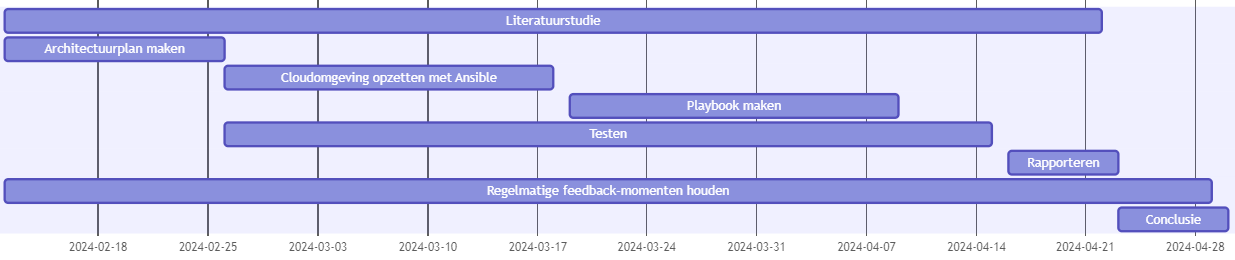
\includegraphics[width=\textwidth]{graphics/gantt.png}
  \caption{Gantt chart}
  \label{fig:gantt}
\end{figure}

%---------- Verwachte resultaten ----------------------------------------------
\section{Verwacht resultaat, conclusie}%
\label{sec:verwachte_resultaten}

De te verwachten resultaten zijn dat dit onderzoek realistisch is en zal bijdragen aan de zoektocht van Aware. Het Proof of Concept is slechts een 
simplistische simulatie van hoe het er aan de werkelijkheid aan toe zou gaan. Het moet bewijzen dat het een mogelijke oplossing is 
voor het probleem en het hoeft daarom niet het finale product zijn.

\section{Discussie, conclusie}
\label{sec:Discussie-conclusie}
Om te bepalen of het Proof of Concept waardig is, wordt het vergeleken met de huidige strategie binnen Aware, waarbij klanten handmatig worden 
opgezet. Dit vergelijkingsproces is essentieel om verschillende aspecten grondig te evalueren, waaronder schaalbaarheid, tijd en 
gebruiksgemak. Door deze factoren te onderzoeken en te analyseren, kan er een dieper inzicht worden verkregen in de potentiële voordelen en mogelijke 
beperkingen van het voorgestelde concept.



%%---------- Andere bijlagen --------------------------------------------------
% TODO: Voeg hier eventuele andere bijlagen toe. Bv. als je deze BP voor de
% tweede keer indient, een overzicht van de verbeteringen t.o.v. het origineel.
%\input{...}

%%---------- Backmatter, referentielijst ---------------------------------------

\backmatter{}

\setlength\bibitemsep{2pt} %% Add Some space between the bibliograpy entries
\printbibliography[heading=bibintoc]

\end{document}
